%!TEX root = ../dissertation.tex

\chapter{What is conceptual complexity?}
\label{chapter:complexity}

The studies in Chapter 2 provide evidence for a regularity between word length and a dimension of word meaning, complexity. In these previous studies, we operationalized the notion of complexity by manipulating the visual complexity of objects in terms of number of component parts. We found that the number of parts  positively correlated with participants' study time in a memory task, providing additional evidence that object complexity was psychologically relevant. Furthermore, we found that the notion of conceptual complexity extended beyond the visual domain to abstract word meanings in natural language. This finding points to a theory of conceptual complexity that is more general than simply the number of visual parts associated with an object.  Notably, however, this work leaves open the important question of what exactly this theory is---what makes one meaning more conceptually complex than another? Here we try to more directly address this question. 

To formalize the notion of complexity, we adopt an information theoretic approach \cite{shannon1948}.\footnote{Note that our discussion of Information Theory here differs from that in Chapter 2 in terms of the domain that the theory is being applied to. In Chapter 2, we appeal to Information Theory to understand the length of words in a communication system. In this chapter, we appeal to the same theory but apply it to  concepts. } The central idea of Information Theory is that, within a communication channel, each meaning $m$ is communicated with probability $p$, such that the amount information conveyed by each occurrence of $m$ is $-log(p)$. Critically, if it is assumed that the overall length of the code in the communication channel is minimized, then meanings should be assigned to codes in a particular way: Less probable meanings should be assigned to longer codes. By making these assumptions, we establish a fundamental link between the amount of information in a code, its probability of occurrence and its length. In our work here, we appeal to this framework to derive a metric of complexity: More complex codes are longer (i.e.\ less compressible), less probable, and contain more information.\footnote{This relationship is reflected in the idea of minimum description length proposed by Kolmogorov and others: In a maximally compressed code, more complex codes are longer.}

Information Theory thus provides a  starting point for evaluating the complexity of a concept by providing a quantitative measure. This proposal is inspired by work on the representation of objects in visual short term memory. To quantify the amount of information in a visual stimulus, \citeA{alvarez2004capacity} measured how long participants took to identify the presence of a visual stimulus among an array of  non-targets. They then used a change detection task to determine the threshold for the number of objects that participants could correctly identify a change in over a short interval of time. Critically, they found that the search rate of a visual stimulus was positively correlated with the memory capacity for that stimulus in the change detection task.  This work suggests that the capacity of visual working memory is in part determined by the amount of information contained within the visual stimuli: Objects that contain more information, as indexed by search rate, are more complex and thus are less compressible in memory. If we apply this same approach to concepts, the central idea is that a concept will be more complex if it contains more information. 

%We define a concept as containing more information if it is defined by more primitives. 

Notably, this proposal is closely related to the Classical Theory of concepts in the philosophical and psychological literatures  \cite{laurence1999concepts}.  A concept in the Classical Theory is defined by a rule, or definition, composed of a structured set of conceptual primitives. These definitions are typically considered deterministic of category membership, but more recent work has considered this theory in a probabilistic framework \cite{goodman2008rational}. To understand this view, consider the geon stimuli from Chapter 2:  If we assume that a primitive ``unit" is equivalent to a geon,  then an object composed of a sphere and cone has a conceptual complexity of two, and an object composed of only a sphere, has a conceptual complexity of one. 

The Classical Theory has been productively instantiated with Boolean concepts and first-order logic \cite{shepard1961learning,feldman2000minimization,goodman2008rational}.  In this  framework, there are a set of primitive concepts, or predicates, that are represented by binary features, and a syntax for combining them given by first order logic.  For example, consider the concept if \textsc{mother}: If \textsc{female} and \textsc{has\_child} were primitives in the representational language, then  \textsc{mother} would denote the set of people where both primitives were true. 

The information theoretic measure of complexity falls straight-forwardly out of this formulation: Concepts defined by more primitives are more complex \cite{shepard1961learning,feldman2000minimization,goodman2008rational}. In the  above example, then, the complexity of the concept  \textsc{mother} would be two. Consistent with this proposal, there is evidence to suggest that the difficulty of acquiring a concept scales with its conceptual complexity: Concepts that are more difficult to learn tend to have longer definitions \cite{shepard1961learning,feldman2000minimization}.

%In the case of concepts, it is not a priori obvious what representational model the cognitive system uses to compress information.  
%An important issue for this theory of concepts is identifying a general set of conceptual primitives.

The central challenge, however, in defining conceptual complexity in information theoretic terms is to define the model, or primitives, over which compression occurs. This is because the metric of complexity depends on the representational model. In other words, what counts as ``one unit" of code depends on the representational model that is assumed. The representational agnosticism of Information Theory implies that a meaning that is relatively more complex in one representational model may be relatively less complex in another, or that  complexity in one representational model may be entirely unrelated to conceptual complexity.

Although defining the representational model of the cognitive system might rank among the deepest challenges for cognitive science, some work has attempted this task. A body of research has sought to understand the innate conceptual primitives in young children (``core knowledge;" Kinzler \& Spelke, 2007). \nocite{kinzler2007core} The proposed set of concepts in this work, however, is restricted to those present only  in early development (e.g., ``agent"), and is therefore not suitable for the broad scope of our current project.  Wierzbicka and colleagues (1996) have also  sought  to identify conceptual primitives, but with a more general focus.  \nocite{wierzbicka1996semantics} This work compares lexical systems across languages  to identify common primitives. The hypothesis is that there exists universal and innate semantic primitives which are the building blocks of meaning in human language. Under this view, all meanings can be derived from a set of numerable semantic primitives and a syntax for combining them.

\begin{table}[t]
\footnotesize
\centering
\begin{tabular}{l l l l  }
 \toprule
 \textbf{Study} &  \textbf{Description} & \textbf{Representational Level}  \\
 \toprule

1  & Descriptions of novel, real objects & type   \\
2  & Definitions of low frequency, real words & type \\
3  & McRae et al.\ (2005) feature norms & type  \\
4  & Concept associates & type    \\
5  & Concept facts & type  \\
6  & Exemplar frequency& token   \\
7  & Exemplar variability & token  \\
 \bottomrule
\end{tabular}
\caption{Summary of studies.}
\label{tab:complexity_pred_summary_table}
\end{table}



 
A related issue to the nature of the representational model is the ontological status of the units over which compression occurs. In particular, whether compression occurs at the type or token level \cite{peirce}. The type level describes an abstract representation, and is most consistent with the ``rule" or ``definitional" nature of the concepts posited by the Classical Theory. In contrast, the token level of representation concerns that which is directly observable; instances of concepts in the real world.  The token level is most closely aligned with the Statistical View of concepts, particularly Exemplar and Prototype Theories in cognitive science  \cite{laurence1999concepts}. Under this view, concepts are represented in terms of actual exemplars observed, either by directly storing exemplars or by computing summary statistics over exemplars. If the cognitive system compresses information at the level of tokens, we might expect, for example, a concept with more observed exemplars to be more conceptually complex. 

In order to understand the nature of conceptual complexity, in this chapter we explore a number of different hypotheses about the model over which the cognitive system might compress meaning. Broadly, in Studies 1-5 we consider a compression model over the level of types, and in Studies 6 and 7 we consider a compression model over the level of tokens (see Table~\ref{tab:complexity_pred_summary_table} for a summary of the studies). In Studies 1-4, we explore whether the definition length of a concept  is related to the length of the label denoting that concept. In these studies, we assume that words denote conceptual units, such that concepts associated with longer linguistic definitions are  more complex. In Study 5, we ask whether the representational model is related to several different culturally relevant facts associated with a concept. Finally, in Studies 6 and 7, we ask whether the frequency and variability of the exemplars of a concept are related to conceptual complexity.  Across all seven studies, we find positive evidence only in support of the hypothesis that number of conceptual primitives, measured linguistically, is related to conceptual complexity.


%In this chapter, we consider two broad hypotheses about the ontol

%In Studies 1-4, we assume that words are either proxies for or are the primitives of the representational model. In Studies 
%Motivated by the Classical View of concepts,

 %While each of these views is consistent with a wide range of theories, we consider each view here in its most general form. We then apply Information Theory to each view of concepts and ask what would make one concept more complex than another, assuming the representational framework of that theory. Briefly, for the Classical View, a more complex concept is one with a longer description length. 

 

%type vs. token
%Representative complexity -for what purpose over which model over which compression occurs
%experience
%Hamming
%We see our goal as not  to distinguish between these  views, nor even that they are incompatible with each other \cite<e.g.,>{murphy2015there,briscoe2011conceptual}. Rather, we consider each of these views as paradigms, in a Kuhnian sense, and ask whether these frameworks can inform our understanding of conceptual complexity when considered in the context of Information Theory. Our approach will be to observe variability in the complexity of meanings as defined within a particular theory of concepts, and ask whether this variability is related to the length of the word that meaning is mapped to. Evidence that a manipulation of conceptual complexity is related to word length would shed light on the underlying construct of conceptual complexity.  

%In what follows, we review previous work related to each broad view of concepts---Classical and Statistical---followed by  a series of empirical studies testing  predictions of each view. In total, we conduct seven studies exploring various predictions these theories (see Table~\ref{tab:complexity_pred_summary_table} for a summary of our studies). We conclude with a brief summary of our results. 




%``length of the shortest Boolean formula logically equivalent to the concept"

%- Evidence consistent with that: Feldman (Boolean) - learning difficult

%- Issue: where do primitives come from? Might be related to experience. If we new what they were


%\cite{laurence1999concepts,anaki2009familiarity,feldman2016simplicity,goodman2008rational,haskell2011linguistic,lupyan2008conceptual,feldman2000minimization}

%Psychological metrics of complexity - trasnfer vs. recognition. 

%If, however, we assume a different representational framework, we might code this same object with a single conceptual primitive, ``ice cream cone."

\section{Experiment 1: Descriptions of objects}
In Chapter 2, we presented participants with novel, real objects and measured their complexity through explicit judgements (Exp.\ 4; pg.\ \pageref{ch2-4}) and study time (Exp.\ 8b; pg.\ \pageref{ch2-8b}). Both of these measures showed variability, suggesting that these objects differed in their complexity.  In Experiment 1, we consider this result in the context of an information theoretic view of concepts. In particular, if the cognitive system's model of representation is related to words, then a more complex concept should be one with more words associated with its meaning. In this experiment, we reasoned that, if true, these primitives should be reflected in participants linguistic descriptions of the objects. More specifically, we predicted that objects rated as more complex and studied longer in Exp.\ 4 and 8b should also be described with longer descriptions. We test this prediction here by asking participants to produce written linguistic description of the objects.

\subsection{Methods}
\subsubsection{Participants} 
In this and all subsequent experiments, participants were recruited on Amazon Mechanical Turk and received US \$0.15-0.50 for their participation, depending on the length of the task. 60 participants completed this first experiment.
\subsubsection{Stimuli}  
We used the same set of 60 novel real objects as in Chapter 2 (Fig. \ref{fig:realobjs}; pg.\ \pageref{fig:realobjs}).
\subsubsection{Participants} 
On each trial, we presented a single object and the following instructions:  ``Look at the object below. Imagine you just received this object as a gift. Describe what the object looks like to a friend." Participants then entered their description in a text box below the object.

Each participant described 10 objects in total. Five objects were from the top quantile (high complexity) and 5 objects were from the bottom quantile (low complexity). Order of objects was randomized across trials.

\subsection{Results and Discussion}


\begin{table}[t!]
\centering

\begin{tabular}{ll}
\toprule
\multirow{6}{*}{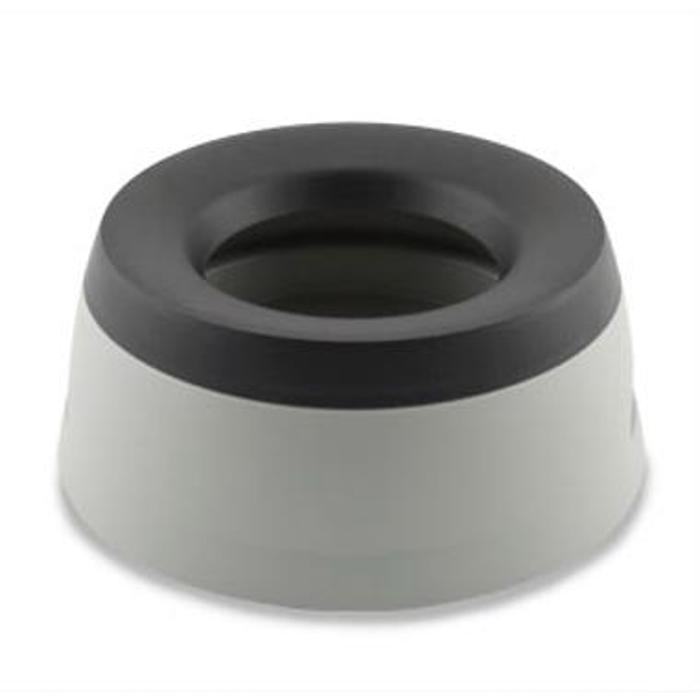
\includegraphics[width=2cm]{figs/obj_29_p2.jpg}} & \textbf{Low-complexity object}                \\
\toprule
                   & ``cup holder"                                   \\
                   & ``it is a bowl with a black portion on top"      \\
                   & ``football kicker's stand"                      \\
                   & ``a hole type thing"                              \\
                   & ``it looks like an ash tray, but a bit shallow" \\
                   & ``looks like a dog bowl" \\
 \bottomrule
~ & ~ \\
  \toprule
\multirow{6}{*}{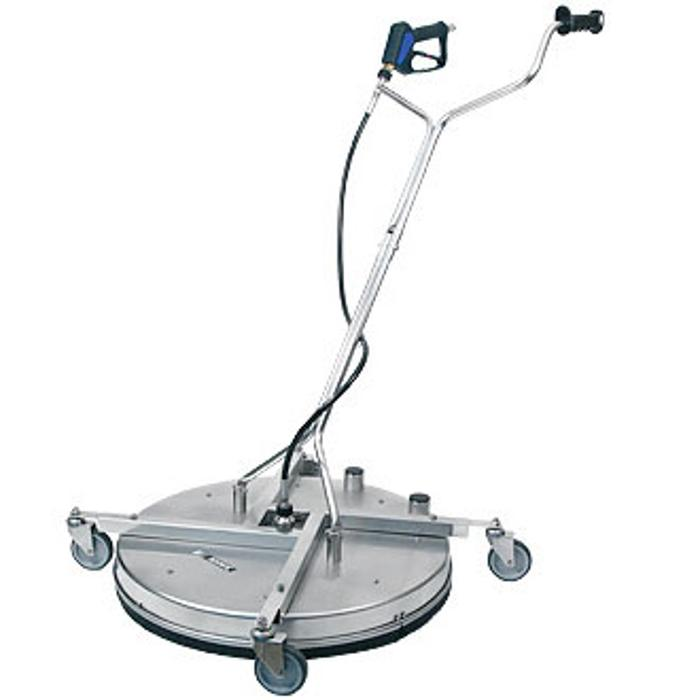
\includegraphics[width=1.8cm]{figs/obj_27_p2.jpg}} & \textbf{High-complexity object}               \\
\toprule
                   & ``a robotic carpet shampooer"                                   \\
                   & \multicolumn{1}{p{12cm}}{ ``it's a flat silver disk on rollers with what appear to be tall handlebars standing away from it at an angle"}                     \\
                   & ``a pressurized floor buffer on wheels"                                   \\
                   & ``it looks like a high tech metal detector on wheel."                                   \\
                   & ``it kinda looks like a portable lamp"                                \\  
                   & ``it is a machine with a circular stand and wheels, it has a metal handle"\\
   \bottomrule
\end{tabular}
\caption{Sample descriptions of a low- (top) and high- (bottom)  complexity objects.  Overall, descriptions were longer for high-complexity objects.}
\label{tab:sample_obj_descriptions}
\end{table}


Example descriptions for a sample low and high complexity object are presented in Table~\ref{tab:sample_obj_descriptions}. We considered two measures of length:  log number of words and log number of characters. Across objects, the mean length of description was  $8.82$ words ($SD = 1.14$) and $36.31$ characters ($SD = 4.69$).

 \begin{figure}[t!]
 \begin{center}
  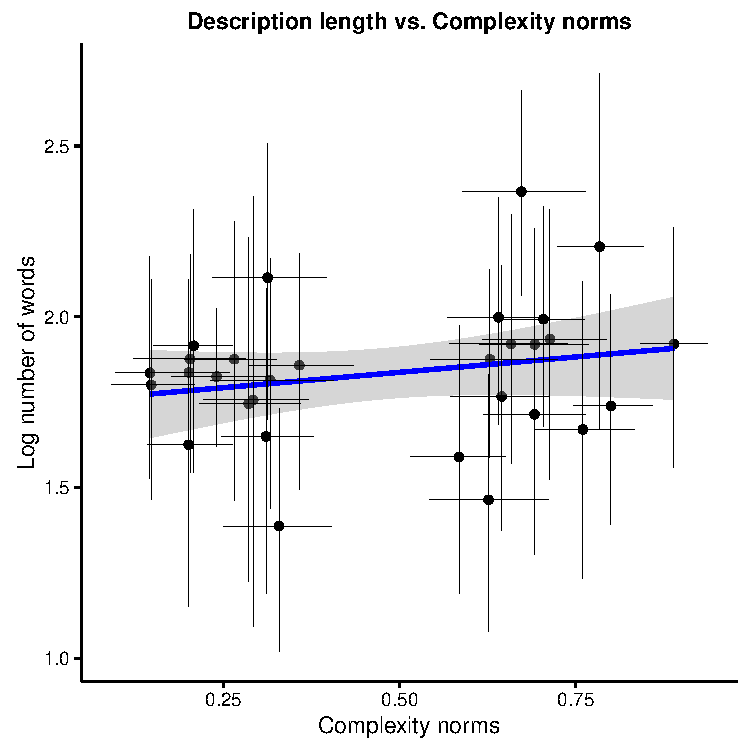
\includegraphics[width=4in]{figs/desc_length_word.pdf}
  \caption{\label{fig:desc_length} Relationship between description length and complexity norms. Error bars show  95\% confidence intervals.}
 \end{center}
\end{figure}


The key question was whether the description length was related to the psychological correlates of complexity measured in Chapter 2, explicit ratings and study times.
To test this question we fit a  linear mixed-effect model predicting log number of words with complexity norms as a fixed effect, and a second model predicting log number of words with study times as a fixed effect. As evident from Table~\ref{tab:sample_obj_descriptions}, participants varied considerably in the  syntactic construction of their descriptions as well as overall  length, making it important to control for this variability using a  mixed-effect model. The random effect structure included by-participant intercepts and by-trial slopes. There was a reliable relationship between log number of words and  complexity norms ($\beta=.2$, $t =2.8$; Fig~\ref{fig:desc_length}), and between log number of words and log study time ($\beta=.59$, $t =3.07$). The same pattern held for log number of characters. 

This result suggests that linguistic representations, in particular, words, may be related to the the coding model of the cognitive system for conceptual complexity.

\section{Experiment 2a: Definitions of words}
Experiment 1 suggested objects that appear visually more complex are described with longer descriptions. The studies in Chapter 2, however, suggest that the construct of conceptual complexity extends beyond visual complexity to abstract word meanings. This predicts that the length of a dictionary definition of a word should be correlated with the conceptual complexity of its meaning. In light of the complexity bias observed in Chapter 2, we also predict that words with more complex definitions should be longer and have definitions that are rated as more complex. In Experiment 2, we tested these predictions by presenting participants with the definition of low frequency English words  and asking them to rate the conceptual complexity of the definition.

We selected low frequency words for several reasons. First, because participants were unlikely to know the word associated with the definition, knowledge of a word's length was unlikely to affect the complexity judgement. Second, because the words were uniformly low frequency, this reduced the possibility that differences in word length were due to frequency, rather than conceptual complexity. Finally, because participants were unlikely to know the words, we could conduct a follow-up experiment (Exp.\ 2b) probing judgements about the length of a meaning's word, without knowledge of the English word interfering with this judgement.

\subsection{Methods}



\begin{table}[t!]
\centering

\begin{tabular}{ll}
\toprule
\textbf{Word} & \textbf{Definition}                \\
\toprule
   bissextile & ``a leap year"\\
   mussitation  &  \multicolumn{1}{p{12cm}}{ ``movement of the lips as if in speech but without accompanying sound"}    \\
   omphaloskepsis  &  \multicolumn{1}{p{12cm}}{ ``contemplation of one's navel as an aid to meditation"}                  \\
   parvis    &  \multicolumn{1}{p{12cm}}{ ``a court or enclosed space before a building"}                               \\
   sniddle      &  \multicolumn{1}{p{12cm}}{ ``long coarse grass"}     \\
   zarf     & \multicolumn{1}{p{12cm}}{ ``a holder, usually of ornamental metal, for a coffeecup without a handle"}                                 \\

 \bottomrule
\end{tabular}
\caption{Sample definitions of real English words used in Experiment 2.}
\label{tab:sample_word_defs}
\end{table}
\subsubsection{Participants}
200 participants completed the task.
\subsubsection{Stimuli}
We selected 100 dictionary definitions of low-frequency words (see Table~\ref{tab:sample_word_defs} for examples). 
\subsubsection{Procedure}
The task was identical to Experiment 9 in Chapter 2 (pg.\ \pageref{ch2-9}), except that participants were presented with definitions rather than words. Participants were first presented with instructions describing the norming task:
\begin{quote}
In this experiment, you will be shown the definition of a word and asked to decide how complex the meaning is. A word's meaning is simple if it is easy to understand and has few parts. An example of a simple meaning is ``brick.'' A word's meaning is complex if it is difficult to understand and has many parts. An example of a more complex meaning is ``engine.''
\end{quote}
For each definition, we then asked ``How complex is this definition?,'' and participants indicated their response on a 7-pt Likert scale anchored at ``simple'' and ``complex.'' The first two words were always ``ball'' and ``motherboard'' to anchor participants on the scale. Each participant rated a sample of 10 definitions. 

\subsection{Results and Discussion}
The central prediction is that definitions with more primitives in the definition, operationalized as the length of the definition, should be rated as conceptually more complex. To test this prediction, we fit a linear mixed-effect model predicting complexity ratings with log number of words in the definition as a fixed effect. The random effect structure included by-participant intercepts and by-trial slopes. As predicted, there was a strong relationship between complexity ratings and log number of words ($\beta=1.50$, $t =27.94$). The same pattern held for log number of characters.

A secondary prediction is that there should be a relationship between the length of the definition and the length of the word: If languages encode the conceptual complexity of a word's meaning in the length of the word, longer words should be associated with longer definitions. This prediction was not supported ($r=.05$, $p =.59$). Finally, we should also expect that  longer words should be associated with definitions rated as more complex. We fit the same mixed-effect model as above to test this prediction, except with log number of characters in the word as a fixed effect. There was a significant relationship between word length and rating judgements ($\beta=.52$, $t =2.86$), suggesting more complex definitions are associated with longer words. However, in a model with both word length and definition length as fixed effects, word length was no longer a reliable predictor of complexity ratings ($\beta=.18$, $t =1.19$).

In sum, we find a strong relationship between definition length and conceptual ratings: Longer definitions, with more primitives, are rated as more complex. We do not, however, find the predicted relationship between the conceptual complexity of the definition and word length, as would be predicted by the studies in Chapter 2.  One possible explanation for this null finding is that participants' complexity ratings were driven by the linguistic complexity of the definition, rather than its conceptual complexity. In other words, participants may have  rated longer definitions as more complex {\it because} they were longer, not because they were more conceptually complex. The current design does not allow us to distinguish these two possibilities.

\section{Experiment 2b: Definition mapping}
If definition length is related to conceptual complexity and participants have a complexity bias, we predict that participants should be biased to map more complex definitions on to longer words. In Experiment 2b, we test this prediction in an experiment analogous to the word mapping experiments in Chapter 2. Participants were presented with a meaning---a definition---and asked to guess the translation of the meaning in an alien language from two possible alternative words, one long and one short. 

\subsection{Methods}
\subsubsection{Participants}
200 participants completed the experiment.
\subsubsection{Stimuli}
We used the normed definitions from Experiment 2a. The short novel words contained one syllable, and the long novel words contained three syllables. There were 10 short and 10 long novel words presented in random order. 
\subsubsection{Procedure}
Participants were first presented with the following instructions:
\begin{quote}
In this experiment, you will see the definition of a word. Your job is to guess what the translation of that word is in an alien language. You will make your guess by betting on two possible words in the alien language. Imagine you have a \$100 dollars. To place your bet, assign an amount to each of the words. Your bets must add to 100.
\end{quote}
Participants then viewed a definition and two possible alternative words, one short and one long. Participants selected a response by placing a numeric bet (0-100) under each word.  Each participant rated 10 definitions in total. 

\subsection{Results and Discussion}
Consistent with previous evidence, we found a complexity bias in participants mappings from definition to words: Participants tended to map definitions rated as more complex in Experiment 2a to longer words ($r = .39$,  $p< .0001$). However, there was also a strong correlation between participants bets to longer words and definition length, measured in terms of log number of characters ($r = .82$, $p< .0001$). In an additive linear model predicting bets to the long word with both complexity norms and definition length, definition length ($\beta=3.81$, $t =2.64$, $p<.01$) was a significant predictor of bets, but complexity norms were not ($\beta=1.02$, $t =1.38$, $p=.17$). 

While this result is consistent with a complexity bias, as well as the pattern of complexity predicted by a linguistic model of representation for compression, it is difficult to make strong causal inferences from these data. The fact that definition length accounts for more variance in bets than complexity norms suggests that it may be linguistic complexity, rather than conceptual complexity that is driving this bias. This result may simply reflect participants bias to map long definitions to long words. While a positive finding, this result does not speak to the claim directly that it is {\it conceptual} complexity per se that is related to definition length and the bias in word length. In Study 3, we try to address this issue more directly. 

\section{Study 3: Feature norms}
Study 3 provides another test of the hypothesis the linguistic model of compression. In this study, however, we measure conceptual primitives through feature norms. This has the advantage of reducing the amount of ``noise" in our measure of primitives by eliminating words that appear in definitions that are not core to the meaning (e.g. prepositions, articles, etc.). Feature norms are collected by presenting participants with the name of a concept (e.g., ``moose") and asking them to produce as many features of the concept as possible (e.g., ``has four legs," ``has antlers"). If we assume that the features participants generate correspond to conceptual primitives in the definition of that concept, then Information Theory predicts that concepts with more  features should be more conceptually complex. If true, we should also expect concepts associated with more features to have longer labels. We test this prediction using a set of previously-collected feature norms.

  \begin{figure}[t!]
 \begin{center}
  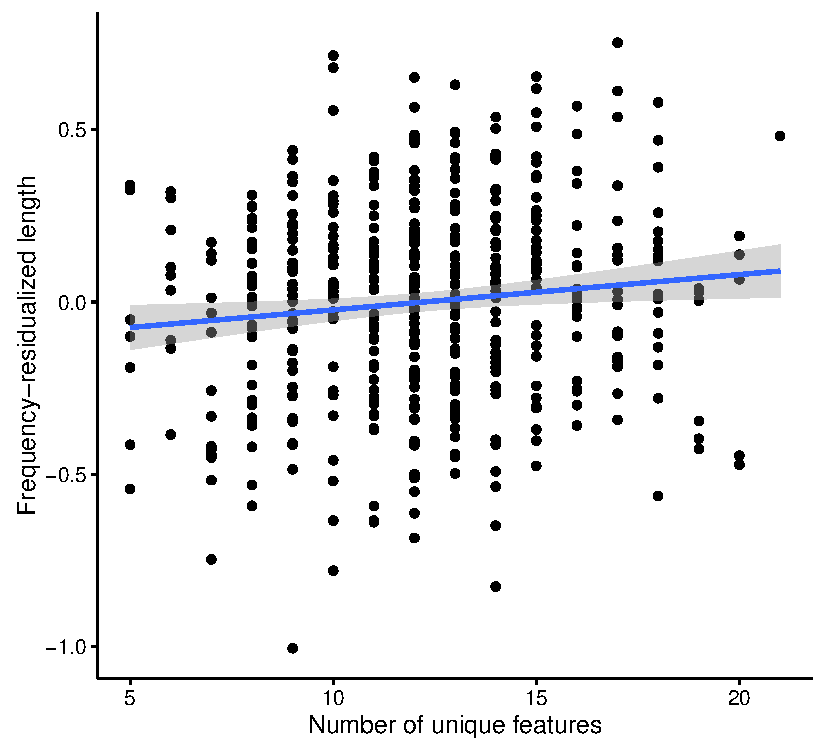
\includegraphics[width=4in]{figs/feature_plot.pdf}
  \caption{\label{fig:feature_plot} Study 3 results: Frequency-residualized word length (measured in log number of characters) as a function of the number of unique features associated with the concept a word denotes. }
 \end{center}
\end{figure}

\subsection{Method}
We analyzed feature norms for a set of 541 nouns \cite{mcrae2005semantic}. For each noun concept, we examined the relationship between the length of the word and the number of unique features participants listed for that concept. A feature was excluded from this measure if it was listed by fewer than 5 of 30 participants or described a taxonomic associate of the concept (subordinate or superordinate). Taxonomic associates were excluded because they are conceptually different than features which describe parts and functions. Word length was measured in terms of log number of characters. We also included spoken frequency of the target noun as a covariate in our models, measured from the Subtlex-us database \cite{brysbaert2009moving}. 

\subsection{Results and Discussion}

We first analyzed the simple correlation between word length and the number of features and found no relationship ($r=-.03$, $p=.54$)  However, spoken frequency is a strong, independent correlate of word length \cite{zipf1936}, and so it is important to control for this variability in measuring the relationship between number of features and word length. We fit an additive linear model predicting word length with both log spoken frequency and number of features.  There was a  relationship between number of features and word length (Fig.\ \ref{fig:feature_plot}): Longer words tended to have more features. Model parameters are presented in Table~\ref{study3amodel}.\footnote{We also fit the same model with the measure of number of features that included taxonomic features. In this model, the relationship between length and number of features was marginal ($\beta=0.08$, $t =1.92$, $p=.06$).} 



% latex table generated in R 3.3.0 by xtable 1.8-2 package
% Mon Oct 10 13:57:56 2016
\begin{table}[t!]
\centering
\begin{tabular}{rrrrr}
  \hline
 & Estimate & SE & t-value & p-value \\ 
  \hline
(Intercept) & 2.2411 & 0.0638 & 35.13 & $<.001$ \\ 
  Num. features & 0.0112 & 0.0043 & 2.59 & $<.01$\\ 
  Log frequency & -0.2626 & 0.0214 & -12.29 & $<.001$  \\ 
   \hline
\end{tabular}
\caption{Model parameters for linear regression predicting word length in terms of number of features, controlling for word frequency.}
\label{study3amodel}
\end{table}

As in Studies 1 and 2, this finding suggests that conceptual complexity may be associated with the number of ``primitive" features associated with a concept, as measured linguistically.

\section{Study 4: Concept associates}
One limitation of Study 3 is the relatively small set of words used in the dataset. In Study 4, we aimed to replicate Study 3 with a larger dataset. We analyzed data from a word-association dataset in which participants were presented with a word and asked to generate three ``related" words. This task differs notably from the feature norms in that participants were allowed to generate any word related to the target, not simply ``features" that describe conceptual parts. While this is a potential limitation of the current approach, we note that the distinction between features and associates is fuzzy. We find  the same pattern as in Study 3: Longer words tend to have more associates. 

In addition, the larger set of cue words in this dataset allowed us to  examine the relationship between the explicit complexity norms collected in  Experiment 9 in Chapter 2 (pg.\ \pageref{ch2-9}) and the number of associates. We reasoned that if the number of associates was related to conceptual complexity these two variables should be positively correlated. This prediction was also supported.

\subsection{Method}
We analyzed an existing dataset containing word associations for  10,050 English words, collected from 73,256 participants \cite{de2013better}. The words included all grammatical classes. In the task, participants were presented with a cue and  asked to type ``the first  three words that came to mind." Each participant completed 15-19 trials. As in Study 3, we used a measure of spoken word frequency from the Subtlex-us database \cite{brysbaert2009moving}. 


\begin{table}[t!]
\centering
\begin{tabular}{llll}
  \hline
 & Log length (char.)  & Complexity norms &   Num. associates  \\ 
  \hline
Log length (char.) &  &  &  \\ 
Complexity norms  &  0.61**** &  &  \\ 
Num. associates &  0.11*    &  0.23**** &  \\ 
Log frequency& -0.54**** & -0.33**** &  0.18**** \\ 
   \hline
\end{tabular}
\caption{Pairwise correlations in Study 4. $p<.05$ = *; $p<.0001$ = ****}
\label{study4corr}
\end{table}

\subsection{Results and Discussion}

We first tested for a relationship between log word length and number of unique associates: Word length was positively correlated with number of associates ($r = .11$, $p< .5$; see Table~\ref{study4corr} for all correlations).  Next, in order to control for the effect of word frequency on length, we fit an additive linear model predicting word length with number of associates and word frequency. Controlling for frequency, the relationship between number of associates and word length remained reliable ($\beta=0.004$, $t =27.34$, $p<.0001$; Fig.\ \ref{fig:associate_plot}).

% latex table generated in R 3.3.0 by xtable 1.8-2 package
% Mon Oct 10 16:07:48 2016


Finally, we examined the relationship between the conceptual complexity norms from  Experiment 9 in Chapter 2  and number of associates. There were 431 words that overlapped between the two datasets. As predicted, there was a strong correlation between the conceptual complexity norms and number of associates: Words rated as more conceptually complex tended to have more associates ($r = .23$, $p< .0001$).




  \begin{figure}[t!]
 \begin{center}
  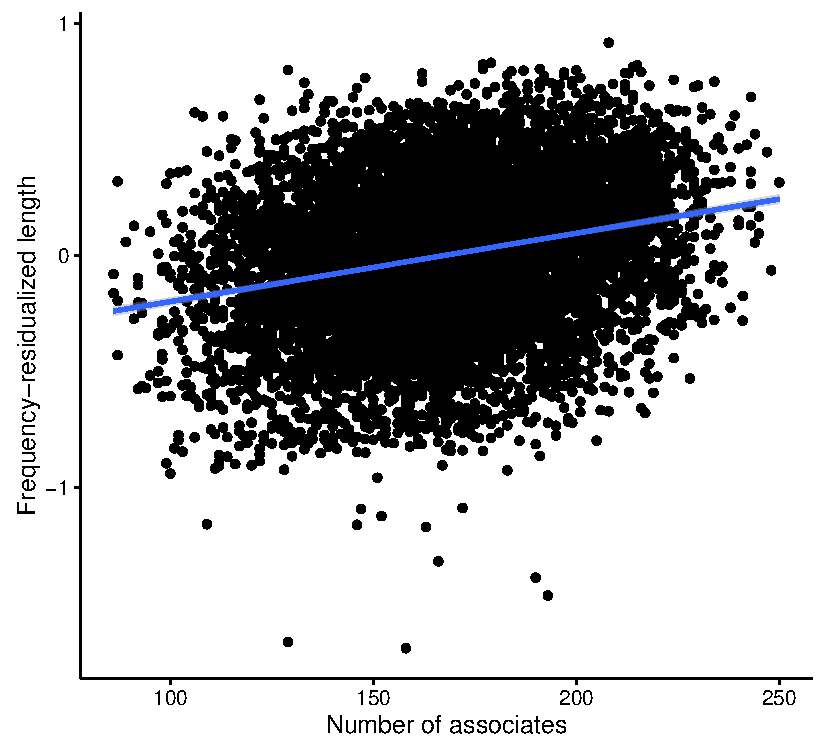
\includegraphics[width=4in]{figs/associate_plot.pdf}
  \caption{\label{fig:associate_plot} Study 4 results: Frequency-residualized word length (measured in log number of characters) as a function of the number of unique associates for a cue word. Each point corresponds to a word. For visualization, outliers three or more deviations above or below the mean were removed.}
 \end{center}
\end{figure} 

%Limit of this test of the classical approach -- assumes features are linguistically based; may not be true.

%we explored the prediction from the Classical View of concepts that more complex concepts are associated with more conceptual primitives. Experiments 1 and 2 suggest that longer linguistic descriptions or definitions of a referent are associated with longer study time of objects and a bias to map that meaning onto a longer word. Studies 3 and 4 more directly tested the hypothesis that conceptual complexity is related to conceptual primitives by measuring the number of unique features associated with a concept. Here, we found that longer words tended to refer to  concepts associated with more features.Taken together, these 



Thus, across four studies, we find support for the notion that the conceptual complexity may be related to the number of conceptual primitives in concept.   Nevertheless, the interpretation of these effects is limited by a number of factors. One issue is  that we  may not have  adequately measured the ``primitives" of conceptual complexity. In all of our studies, we assume that language can be used as a proxy for conceptual primitives. If this is not true, or linguistic representations are a poor proxy for conceptual primitives, then this would limit the interpretability of our findings. Indeed, identifying  conceptual primitives is one of the largest challenges for this view. In addition, this work here does not provide an account of how conceptual complexity might change with experience (e.g. why ``telephone" might become ``phone").  In Study 5, we examine another possible representational model: culturally-relevant facts associated with the concepts. 


%\section{Conceptual complexity under the Statistical View}
%The Statistical View of concepts assumes that leaners acquire concepts inductively from a noisy set of exemplars. Importantly, unlike the Classical View, this view does not posit an underlying set of conceptual primitives or  a theory for how new concepts can be derived from other concepts. Within the Statistical View, there are two major theories: Exemplar and Prototype Theory. Exemplar Theory assumes that a concept is represented as the set of individual exemplars observed of that category, with no additional compression of the concept in long term memory \cite<e.g.,>{medin1978context}. In contrast, the Prototype Theory assumes that a concept is stored as a summary representation, or ``prototype," of the set of observed exemplars of a concept [CITE].
%
%We can operationalize the notion of conceptual complexity within each of these theories by applying the description length criteria of Information Theory. In the case of Exemplar Theory, we  assume that the primitives of representation are individual exemplars. In Information Theoretic terms, this implies that a concept with more exemplars would have a longer ``code" than a concept with fewer exemplars, and thus would be more complex. To understand this prediction intuitively, consider an expert who has observed many exemplars of a concept: A bird expert, for example, would have many stored exemplars of birds as part of the concept  \textsc{bird}. The Exemplar Theory predicts that the bird expert would have an overall more complex representation of the concept \textsc{bird}, relative to a non-bird expert. 
%
%[TO DO] There is some evidence to support this prediction from work showing that observing more exemplars leads to worse memory for overall exemplars
%- More exemplars more transfer; worse memory for individual exemplars (see Omohunder, 1981; King and Newman, 1982)
%Salthouse (1977): more exemplars increases recognition reaction time for letters, but NOT dot patterns (a concept) [same holds for accuracy)
%Difference goes away with only a little bit of exposure
%Argue there is an effect of number of exemplars only early in learning
%\footnote{Evaluate: ease of learning model vs. transfer}
% 
%In the case of Prototype Theory, we can operationalize conceptual complexity by appealing  directly to the statistical framework of the theory: A more complex theory is one with more uncertainty associated with the prototype. To understand how this is related to experience, assume we sample exemplars from the population distribution of exemplars, and represent that sample by a summary representation (a prototype). By the law of large number, our uncertainty about the prototype of the concept becomes smaller as we sample more exemplars. Thus, the prototype theory predicts that as the number of observed exemplars increases, uncertainty about the prototype decreases, and thus its conceptual complexity decreases. This same prediction also falls directly out of an information theoretic account: Objects that appear more frequently are less surprising, and thus less conceptually complex. Notably, this prediction is the opposite of that predicted by the Exemplar Theory: While Exemplar Theory predicts that concepts with high frequency exemplars are more complex, Prototype Theory predicts that concepts with high frequency exemplars are less complex. 
%
%[TO DO]There is also some evidence to support the prediction from the Prototype Theory.
%- Familiarity speeds visual search paradigms (Wang, Cavaneough, Green 1994 ) 
%- named famileiar matters more (Lupyan, 2008)
%
%In addition to the frequency of exemplars, Prototype Theory also makes a prediction about the {\it variability} of exemplars. If we again imagine that we are sampling exemplars from the population distribution of concepts, then we might expect concepts to have different variances around the prototype. With the assumption that learners are estimating the prototype, or mean, of the concept, then greater variance in exemplars implies less certainty about the mean. Thus, higher variance concepts are predicted to be more conceptually complex.
%
%[TO DO]Variability work
%haskell
%Anaki paper -- more experience, faster at responding
%Familairity maters in visual search paradimg (Frith, 1974)

%In Experiments 5-7, we test these predictions about the frequency and variability of exemplars. In Experiment 5, we ask whether the number of observed exemplars is related to conceptual complexity. In Experiment 6, we ask whether conceptual frequency, or markedeness, is related to conceptual complexity.  Finally, in Experiment 7, we ask whether a different dimension---exemplar variability---predicts conceptual complexity. Overall, we find no evidence for the Statistical View of conceptual complexity. 
%we  test the hypothesis that the number of observed exemplars is related to conceptual complexity. However, in the present experiment, we explore the possibility that perhaps raw number of times an exemplar is observed is not the psychologically relevant dimension of frequency. We instead ask whether {\it conceptual} frequency, or markedness, is

\section{Experiment 5: Facts}
While the previous experiments assume that conceptual primitives are related to the number of words in a concept's definition, here we ask whether culturally relevant facts associated with a concept might influence its conceptual complexity. In Experiment 5,  we teach participants facts about novel objects, and then ask them to map those objects to short or long words. We selected four categories of facts  that were intuitive candidates for culturally significant units of compression: Monetary cost, frequency of use, frequency of discussion, and frequency of appearance on Facebook.

\subsection{Method}



\subsubsection{Participants}
120 participants completed this experiment. 
\subsubsection{Stimuli}
All participants were presented with the same eight facts, shown in Table \ref{tab:facts}. Objects were again a sample of the novel, real objects used in Chapter 2, Expts.\ 4-6.  The linguistic stimuli were novel words composed of either 2 (e.g., ``tupa," ``gabu," ``fepo")  or 4  (e.g., ``tupabugorn," ``gaburatum," ``fepolopus")  syllables.

\begin{table}[t!]
\centering

\begin{tabular}{ll}
\toprule
\textbf{Category} & \textbf{Fact}               \\
\toprule
   facebook & ``$\rule{1cm}{0.15mm}$s appear in the background of \{a couple/many\} pictures on Facebook."\\
   money  &  ``$\rule{1cm}{0.15mm}$s cost \{\$4/ \$400\}."   \\
   talk  & ``$\rule{1cm}{0.15mm}$s get talked about once a \{day/year\}." \\
   use    & ``$\rule{1cm}{0.15mm}$s are used once a \{day/year\}."                             \\

 \bottomrule
\end{tabular}
\caption{The eight facts used in Experiment 5. For each of the four categories, there was a low and high frequency alternate (shown in  brackets).}
\label{tab:facts}
\end{table}

\subsubsection{Procedure}
Participants were presented with the following instructions:

\begin{quote}
In this experiment, you will learn facts about objects but the name of the object will be missing. For example, a fact like, ``Mops are used for cleaning the floor," will appear as ``$\rule{1cm}{0.15mm}$s are used for cleaning the floor." After you memorize these facts, you will then be asked to guess the name for each object. 
\end{quote}
Participants  then saw  all 8 facts paired with an object. The facts appeared just as in  Table \ref{tab:facts}, with a blank for the name of the object. Participants were allowed to study the fact-object pairings for as long as they wanted. They then proceeded to a test phase where  each object was shown next to a multiple choice set of all 8 facts. For each object, participants had to select which fact from the training phase was true of that object. Participants were then given feedback about their responses, and repeated the study and test phase until all 8 facts were correctly recalled. 

Next, participants completed a mapping task as in previous experiments. Participants saw a novel word and two objects and were asked to guess which object the word referred to. Each participant completed four mapping trials, two with long words and two with short words. The pairs of objects in each trial were from the same fact category (``facebook," ``money," ``talk," or ``use"). Thus, each trial required participants to make a judgement about the meaning of a word between a low  and high conceptually-frequent object. Order of categories was counterbalanced across participants. Word lengths were randomized across trials. 

\subsection{Results and Discussion}
  \begin{figure}[t!]
 \begin{center}
  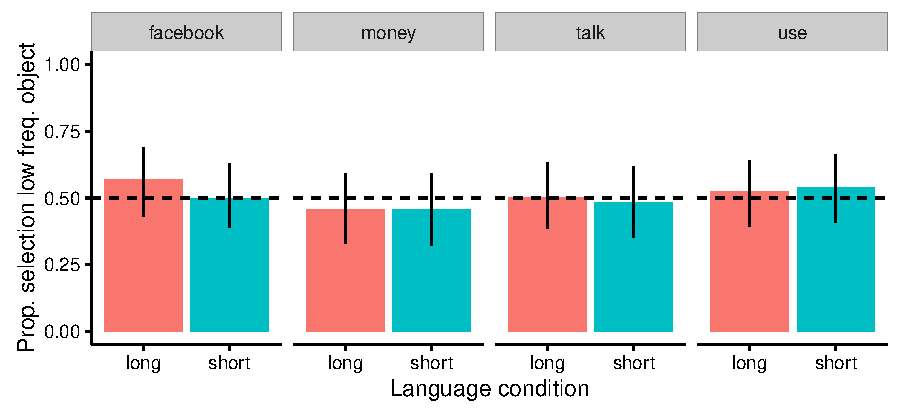
\includegraphics[width=6in]{figs/fact_plots.pdf}
  \caption{\label{fig:fact_plots} Experiment 5 results: Proportion participants selecting the object associated with the low frequency fact as a function of fact category and language condition. See Table \ref{tab:facts} for explanation of fact categories. Error bars are bootstrapped 95\% confidence intervals.}
 \end{center}
\end{figure}
Participants studied and completed the test a mean 2.4 times ($SD = 1.49$).  Across all four categories, there was no evidence that selections to the short or long word varied as a function of the frequency valence of the fact (all ${\chi}^2$$(1) < 3.8$; $p > .5$). Results did not differ as a function of how many times participants studied the facts.  This failure suggests that our facts may not be related to the representational model used by speakers in compressing meaning. 
%In sum, then, across both Experiments 5 and 6, we find no evidence that exemplar frequency, either objective  or psychological, is related to conceptual complexity. Next we turn to a final hypothesis about the nature of conceptual complexity: exemplar variability. With these limitations in mind, 



\section{Experiment 6a: Simultaneous frequency}
Studies 1-5  tested hypotheses about the representational model of complexity at the level of types. In the next two experiments, we  consider representational models over a different level of representation: tokens. In Experiment 6, we ask whether the number of exemplars a participant observes influences the conceptual complexity of the concept. We present participants with either a few or many exemplars of a concept, and then ask participants to map that concept to either a short or long label. If conceptual complexity is related to exemplar frequency, we should expect the number of exemplars observed to influence how a concept is mapped to words of varying length. In particular, if concepts with more exemplars are conceptually less complex, we should expect long words to be mapped to objects that appear less frequently.
%Under the Exemplar Theory, we expect long words to map to concepts with many exemplars, and under the Prototype Theory, we expect long words to map to concepts with few exemplars.

\subsection{Methods}
\subsubsection{Participants}
477 participants completed the experiment.
\subsubsection{Stimuli}
The objects were composed of a single geon, similar to those used in Expts.\ 1-3 in Chapter 2. The novel words were identical to Exp.\ 5.
\subsubsection{Procedure}
We presented participants with 10 objects on a single screen with a cover story that the objects were from a character's box (see Fig.\ \ref{fig:seqfreq_display} for precise text). Participants were required to click on a question mark to reveal each object. There were always two types of objects, one appearing nine times and the other once. Order of presentation was randomized.

After this training phase, participants completed a forced choice mapping task, as in Studies 1 and 5 in Chapter 2 (pg.\ \pageref{ch2-1} and pg.\ \pageref{ch2-5}). We presented a short or long word and asked participants to make a judgment about whether the word referred to the low or high frequency object. Each participant completed a single mapping trial, and word length was manipulated between participants.

 \begin{figure}[t!]
 \begin{center}
  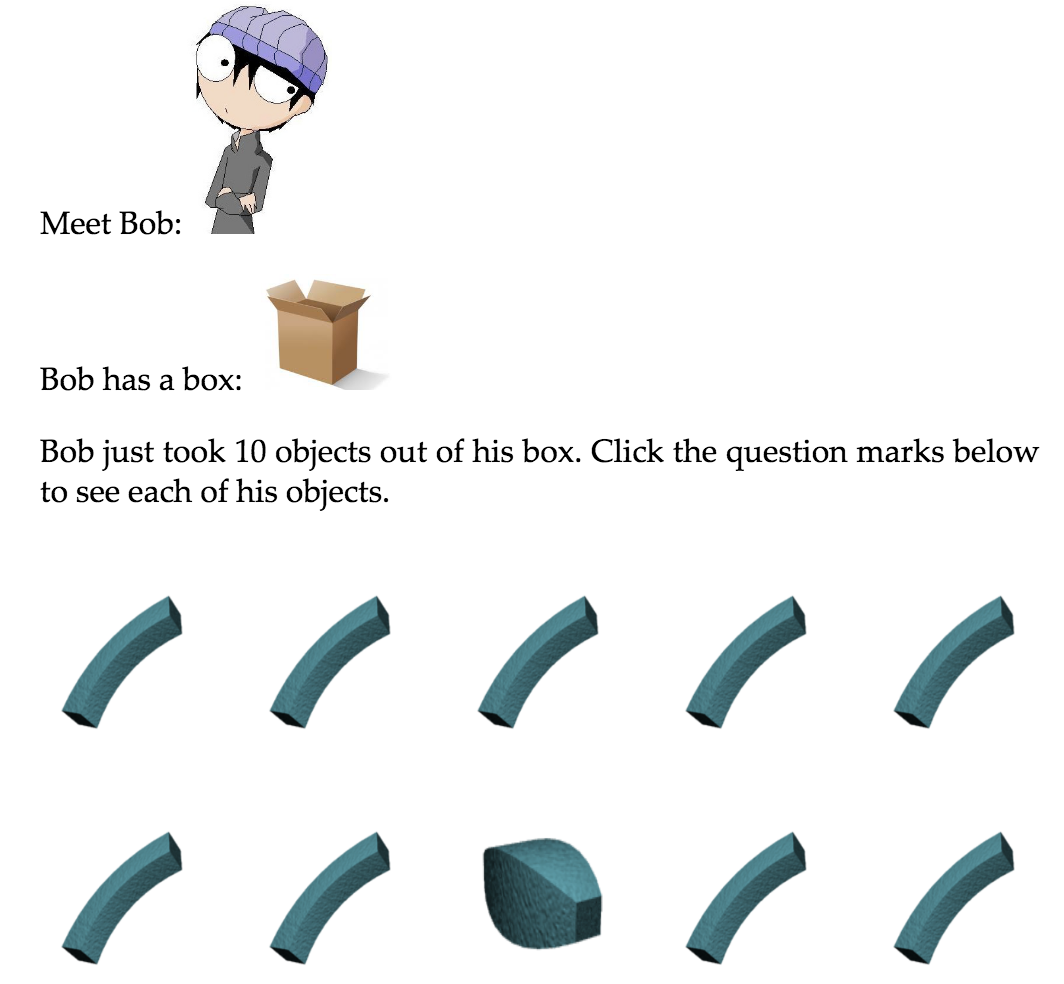
\includegraphics[width=3.5in]{figs/seqfreq_display.png}
  \caption{\label{fig:seqfreq_display} Sample display of the training phase in Experiment 5a.}
 \end{center}
\end{figure}


 \subsection{Results}
 Selections between the two conditions did not differ (${\chi}^2$$(1) = 0.02$, $p = .89$; Fig.\ \ref{fig:freq_plots}, left).
 
  \begin{figure}[t!]
 \begin{center}
  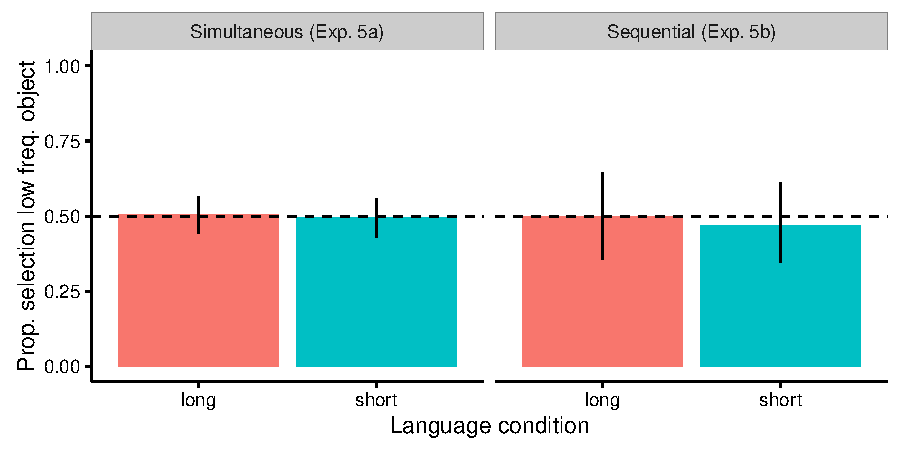
\includegraphics[width=6in]{figs/freq_plots.pdf}
  \caption{\label{fig:freq_plots} Proportion participants selecting the low frequency object as a function of language condition, in Exp.\ 6a (left) and Exp.\ 6b (right). Error bars are bootstrapped 95\% confidence intervals.}
 \end{center}
\end{figure}

\section{Experiment 6b: Sequential frequency}
Given the null finding in Experiment 6a, we next explore whether the timing of the presentation of exemplars affects complexity. Previous work has shown that participants may induce different concepts depending on whether or not exemplars are presented simultaneously, as in Experiment 6a,  or sequentially \cite<e.g.>{spencer2011}. In Experiment 6b, we present exemplars sequentially such that only one exemplar is visible at any given time. 

\subsection{Method}
\subsubsection{Participants}
97 participants completed the experiment.
\subsubsection{Stimuli}
The objects were the set of novel, real objects used from Chapter 2, Expts.\ 4-6. The novel words were identical to Exp.\ 5 and 6a.
\subsubsection{Procedure}
We manipulated object frequency by sequentially presenting objects. Participants saw 60 objects one at a time for 750 ms per object. One object was presented 10 times and a second object was presented 40 times. Ten additional objects were included as fillers, each appearing once. These were included to make the critical manipulation less obvious. Order of presentation was randomized. After this training phase, participants completed a single mapping trial as in Experiment 6a. Word length was manipulated between participants.

\subsection{Results and Discussion}
Selections between the two conditions did not differ (${\chi}^2$$(1) = 0.01$, $p = .92$; Fig.\ \ref{fig:freq_plots}, right). Across Expts.\ 6a and 6b, we find no evidence that the frequency of exemplars is related to the conceptual complexity of objects. 

One possible reason for this null finding might be that we were not successful in manipulating the frequency of tokens in the present experiments. Instead, participants may have perceived our manipulation as repeated instances of the same token. Under this interpretation, our manipulation could be seen as varying the familiarity with a particular token. We tried to force the token interpretation of our objects through the cover story, but this was undermined by the fact that all of the objects were identical. These experiments are thus  suggestive that frequency of tokens is not the coding model for complexity, but a stronger test of this hypothesis would be a manipulation that varied exemplars within a concept. 

\section{Experiment 7: Exemplar variability}
In the final experiment, we forced the token interpretation of our stimuli by presenting participants with several different exemplars of a concept. In this experiment, we test the hypothesis that the coding model for complexity is related to the variability of exemplars:  A concept is more conceptually complex if its exemplars are more variable. We test this prediction by presenting participants with a low and high variability concept and asking them to map a novel word to the concept. If conceptual complexity is related to exemplar variability, we predict that participants should be biased to map a longer word onto a concept with more variable exemplars.

\subsection{Method}
\subsubsection{Participants}
396 participants completed the experiment.
\subsubsection{Stimuli}
The linguistic stimuli were identical to previous experiments. There were four classes of object stimuli (bugs, birds, flowers, and fish). Each participant saw 10 objects from two classes. For each object class, two features varied continuously (e.g. for bugs, body and head size). Size parameters for the low variability objects were  sampled from a low variability distribution, and size parameters for the high variability objects were  sampled from a high variability distribution (see Fig.\ \ref{fig:var_screen_shot} for sample stimuli sets).

  \begin{figure}[t!]
 \begin{center}
  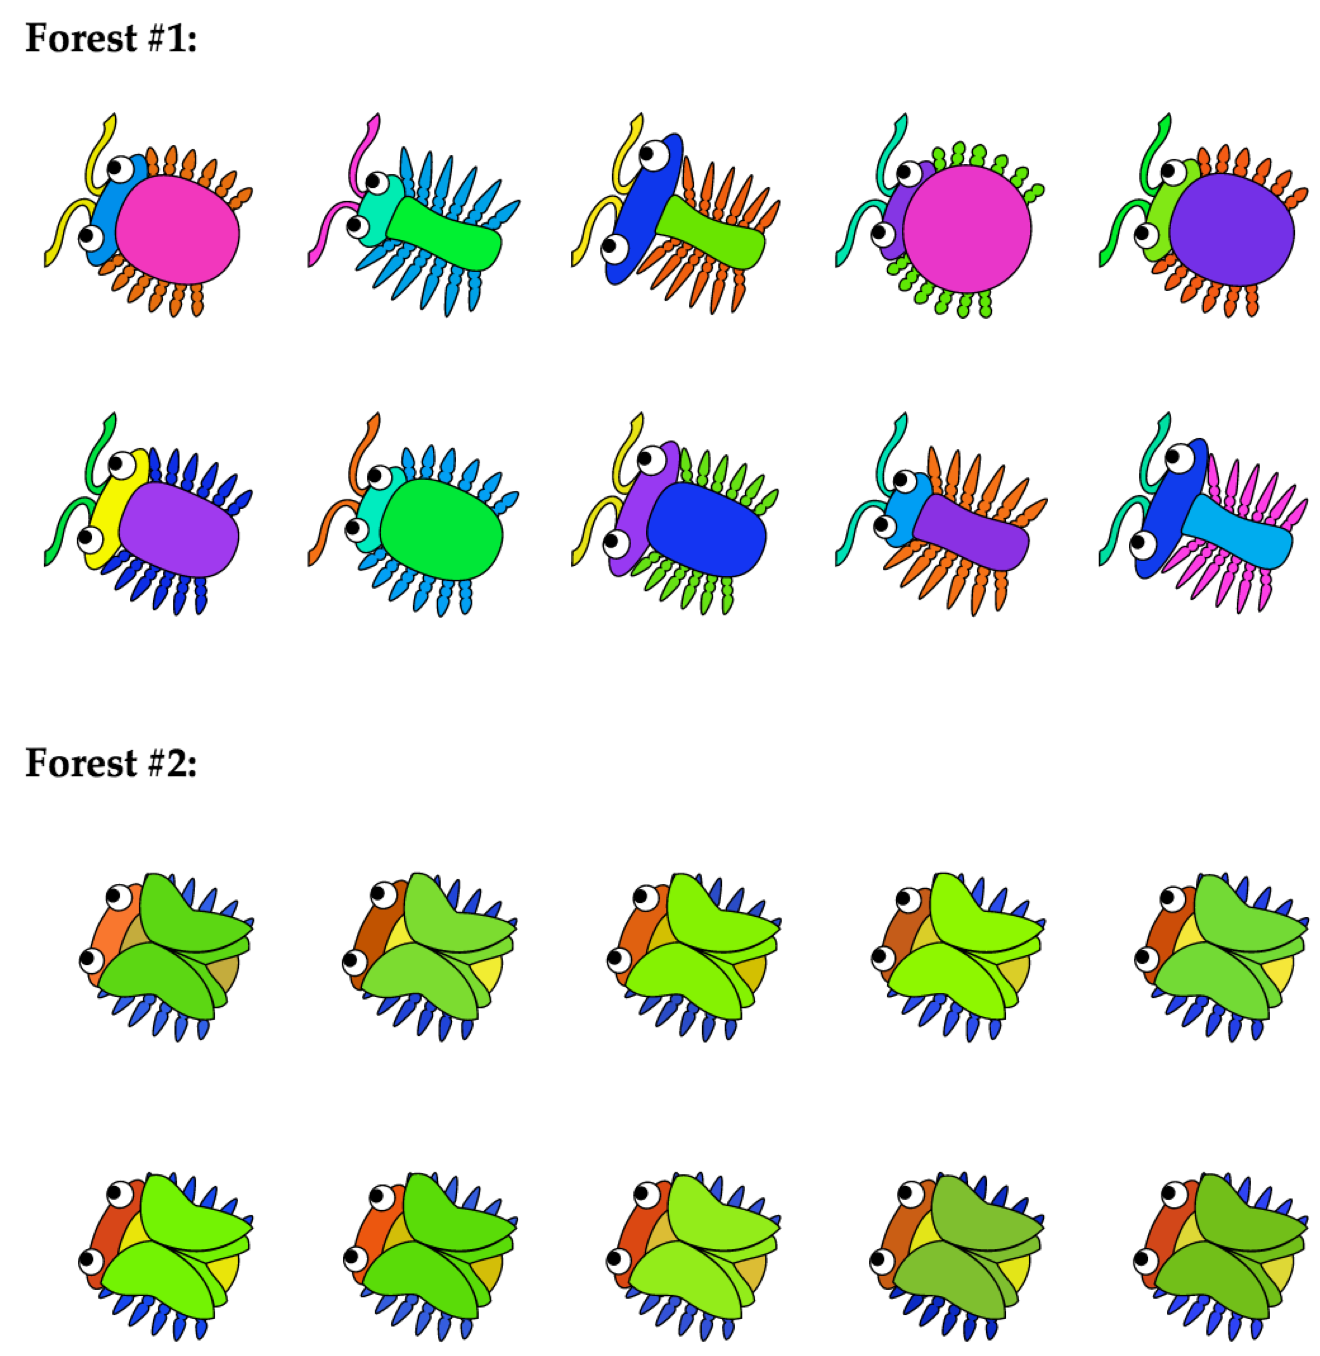
\includegraphics[width=4in]{figs/var_screen_shot.png}
  \caption{\label{fig:var_screen_shot} Example stimuli sets in Experiment 7. High variability bugs are shown on top (Forest \#1) and low variability on bottom (Forest \# 2).}
 \end{center}
\end{figure}

\subsubsection{Procedure}
The procedure was identical to Exp. 6a, with the exception of the training display. During the training phase, participants were given the following instructions:

\begin{quote}
In the country of Desodonia, there are two different \{forests/forests/fields/lakes\}. Each \{forest/forest/field/lake\}  is home to a different kind of \{bug/bird/flower/fish\}. To see some of the \{bugs/birds/flowers/fish\} in each \{forest/forest/field/lake\}, click the question marks below.
\end{quote}

They then saw two 5-by-2 grids of question marks corresponding to two different forests, fields, or lakes. Participant revealed the object by clicking on the question mark. After all question marks had been clicked, the final display appeared as in Fig.\ \ref{fig:var_screen_shot}. Following this training phase, participants advanced to a single word mapping trial as in Exp. 6a. One of the referent alternatives was an exemplar from the low variability concept, and the other was an exemplar from the high variability concept. Word length was manipulated between subjects.

  \begin{figure}[t!]
 \begin{center}
  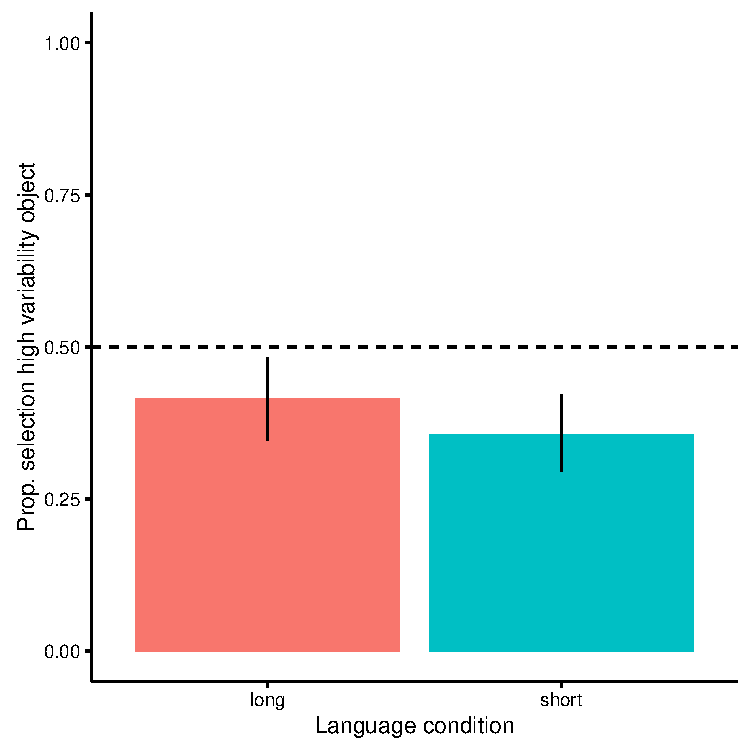
\includegraphics[width=4in]{figs/var_results.pdf}
  \caption{\label{fig:var_plot} Experiment 7 results: Proportion participants selecting the object associated with the high variability fact as a function language condition.  Error bars are bootstrapped 95\% confidence intervals.}
 \end{center}
\end{figure}


\subsection{Results and Discussion}

Selections of the high variability object did not differ as a function of word length (${\chi}^2$$(1) = 1.12$, $p = .29$; Fig.\ \ref{fig:var_plot}). However, 70 participants failed to correctly recall which category member was from the high-variability category, suggesting that participants may not have even noticed the critical manipulation. Nevertheless, even with these participants excluded, there was no difference between conditions (${\chi}^2$$(1) = .05$, $p = .82$). We thus find no evidence to suggest that exemplar variability is related to conceptual complexity.



\section{Conclusion}
In this chapter we sought to understand the nature of the conceptual complexity as reflected in the bias for participants to map longer words to more complex  referents. We used the framework of  Information Theory to quantify conceptual complexity. Critically, however, to develop a predictive theory of conceptual complexity using Information Theory we must identify the  coding model used by the cognitive system to represent meaning. This was the goal of the present chapter.  Across a series of seven studies, we find some support for the possibility that the units of the coding model may be related to linguistic units. We find no evidence that the coding model is related to the representation of exemplars. 

The possibility that language is, or is closely related to, the coding model for complexity is a very intriguing possibility. One implication of  this proposal is that the set of primitive concepts  for a person may change with experience. In particular, the complexity of a concept might reduce when subsets of its primitives are bundled together and labeled \cite{bruner1956austin}. In other words, a concept that is initially complex could reduce in  complexity, such that it itself becomes an atomic unit in other concepts.  This proposal is consistent with a body of literature suggesting advantages in concept learning for labeled as opposed to unlabeled categories \cite<e.g.>{balaban1997,lupyan2007,sloutsky2001}. 

%However, there is reason to think that other aspects of experience might affect the conceptual complexity of concepts since the length of words can change over time. For example, the word ``telephone" has become more typically ``phone" in standard usage. This type of  diachronic reduction in word length may be due to factors  unrelated to conceptual complexity (e.g.\ frequency of usage), but it might also reflect a decrease in conceptual complexity due to experience, beyond simply tokening the concept. Our work here does not directly address the character of the underlying  primitives, nor whether they are universal or innate or change over time. Rather, it assumes only that such units exist for a speaker and that lexical meanings can vary in the number of their compositional primitives. 


In sum, the present set of studies  suggest that Information Theory may be a productive framework for quantifying complexity in the domain of concepts. The ultimate utility of this approach, however, relies on identifying the  coding model used by the cognitive system, and this is a very challenging task. Nevertheless, the studies here begin to answer this question by pointing to linguistic representations as a  potential correlate of the coding model.

%the most productive framework for describing the notion of conceptual complexity may be conceptual primitives. Nevertheless, there is still much work to be done to understand what these primitives are.  Thus, a central challenge for this work moving forward will be to provide an account of the origin and nature of conceptual primitives and how they change over time, both ontogenetically and phylogenetically.










